\documentclass{beamer}

\usepackage[utf8]{inputenc}
\usepackage{hyperref}

\usetheme{Berkeley}
\beamertemplatenavigationsymbolsempty
\setbeamertemplate{headline}{}
 
\title{Importing data into FoodChain-Lab 2}
\date{}
 
\begin{document}
\maketitle

\section{ }

\subsection{Tasks}
\begin{frame}
	\begin{itemize}
		\item In this part of the tutorial we will do a back- and forward-tracing from the "Frozen Fruit Sales" station.
		\item You can either complete part 1 of the tutorial or directly import the following files into an empty database before starting this tutorial.
		\item Caterer 1 Start: \url{https://github.com/SiLeBAT/BfROpenLabResources/raw/master/GitHubPages/documents/Start_Tracing_Forward_Caterer1.xlsx}
		\item Caterer 2 Start: \url{https://github.com/SiLeBAT/BfROpenLabResources/raw/master/GitHubPages/documents/Start_Tracing_Forward_Caterer2.xlsx}
		\item Caterer 1 Backward: \url{https://github.com/SiLeBAT/BfROpenLabResources/raw/master/GitHubPages/documents/StationBacktrace_request_Caterer 1_-1839649003.xlsx}
		\item Caterer 2 Backward: \url{https://github.com/SiLeBAT/BfROpenLabResources/raw/master/GitHubPages/documents/StationBacktrace_request_Caterer 2_-530502898.xlsx}
	\end{itemize}
\end{frame}
 
\subsection{1}
\begin{frame}
	\begin{center}
  		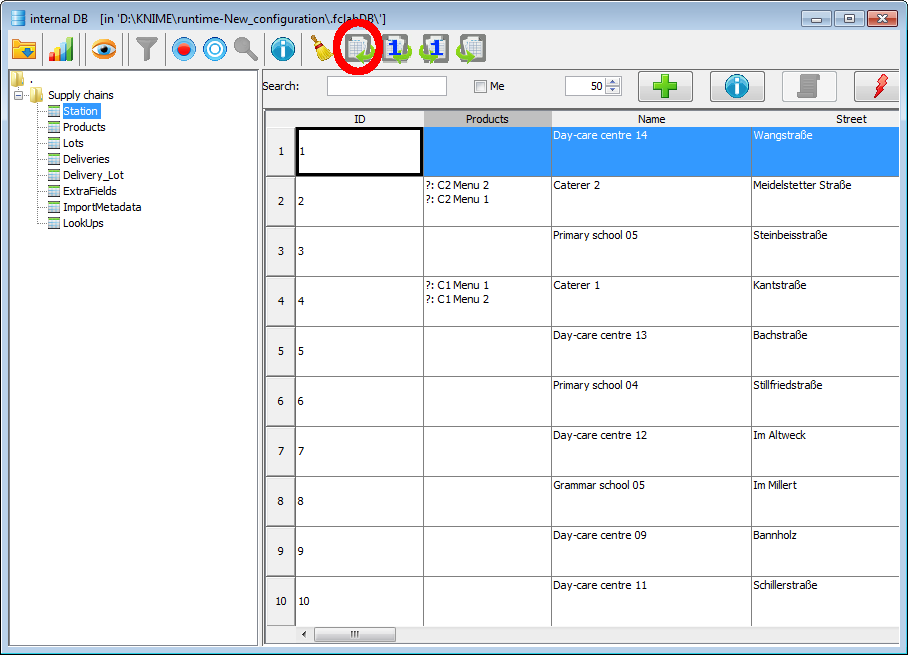
\includegraphics[height=0.6\textheight]{1.png}
	\end{center}
	\begin{itemize}
		\item You should have the database interface open.
		\item Press the button for generating a backtracing template for one station, which is marked by the red circle.
	\end{itemize}
\end{frame}

\subsection{2}
\begin{frame}
	\begin{center}
  		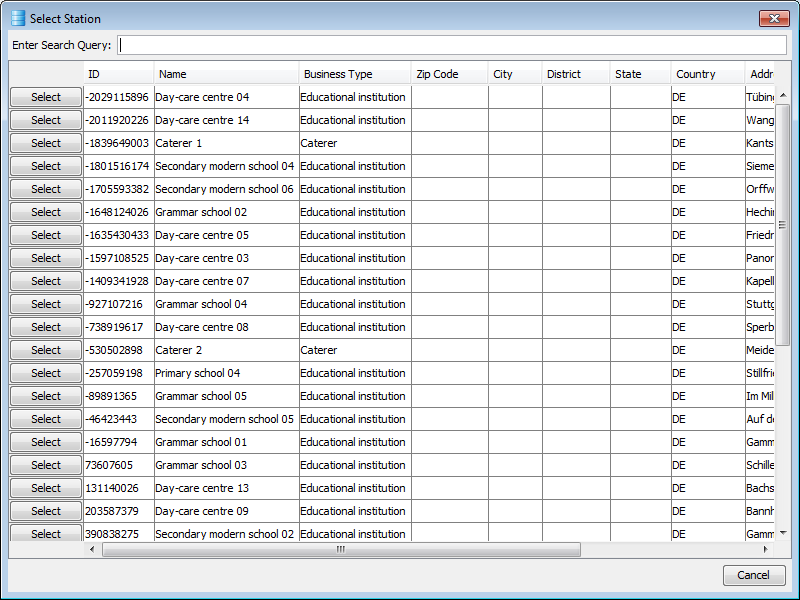
\includegraphics[height=0.5\textheight]{2.png}
	\end{center}
	\begin{itemize}
		\item In the dialog that appears, you can see a table with all stations from the database.
	\end{itemize}
\end{frame}

\subsection{3}
\begin{frame}
	\begin{center}
  		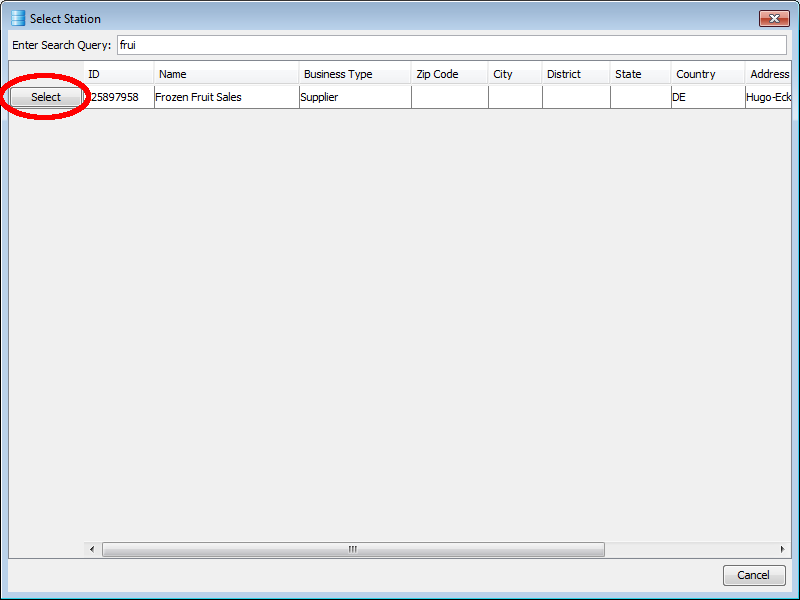
\includegraphics[height=0.5\textheight]{3.png}
	\end{center}
	\begin{itemize}
		\item Type the first letters of "Frozen Fruit Sales" in the search box to search for it.
		\item After typing some letters all other stations should have disappeared. Click on the \textbf{Select} button for "Frozen Fruit Sales".
	\end{itemize}
\end{frame}

\subsection{4}
\begin{frame}
	\begin{center}
  		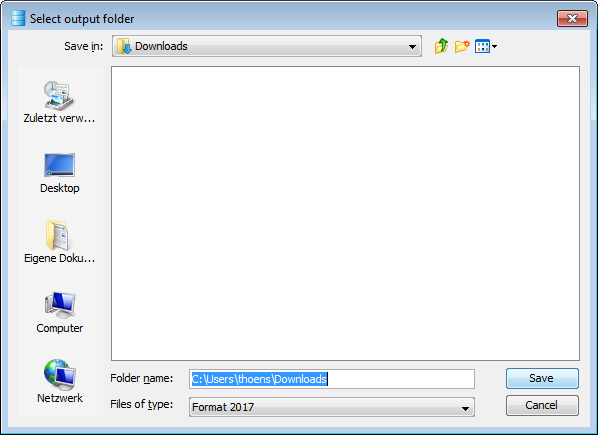
\includegraphics[width=0.8\textwidth]{4.png}
	\end{center}
	\begin{itemize}
		\item In the file dialog that appears, you can specify the folder where the generated template should be saved.
		\item Select the desired folder and press \textbf{Save}.
	\end{itemize}
\end{frame}

\subsection{5}
\begin{frame}
	\begin{center}
  		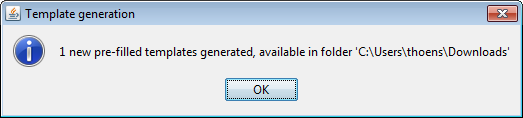
\includegraphics[width=0.95\textwidth]{5.png}
	\end{center}
	\begin{itemize}
		\item You'll be noticed, that one template was generated in the folder you specified.
		\item Press \textbf{OK}.
	\end{itemize}
\end{frame}

\subsection{6}
\begin{frame}
	\begin{center}
  		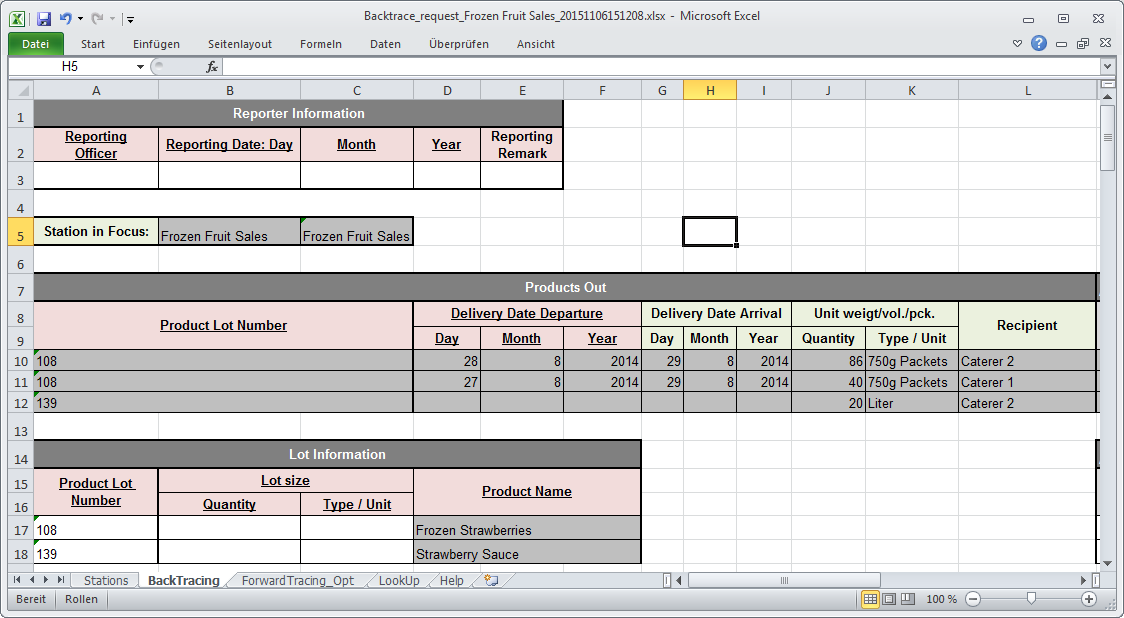
\includegraphics[width=0.95\textwidth]{6.png}
	\end{center}
	\begin{itemize}
		\item Open the generated template "StationBacktrace\_request\_Frozen Fruit Sales\_725897958...".
		\item In the upper part of the sheet you can see the three outgoing deliveries from to "Caterer 1" and "Caterer 2".
	\end{itemize}
\end{frame}

\subsection{7}
\begin{frame}
	\begin{center}
  		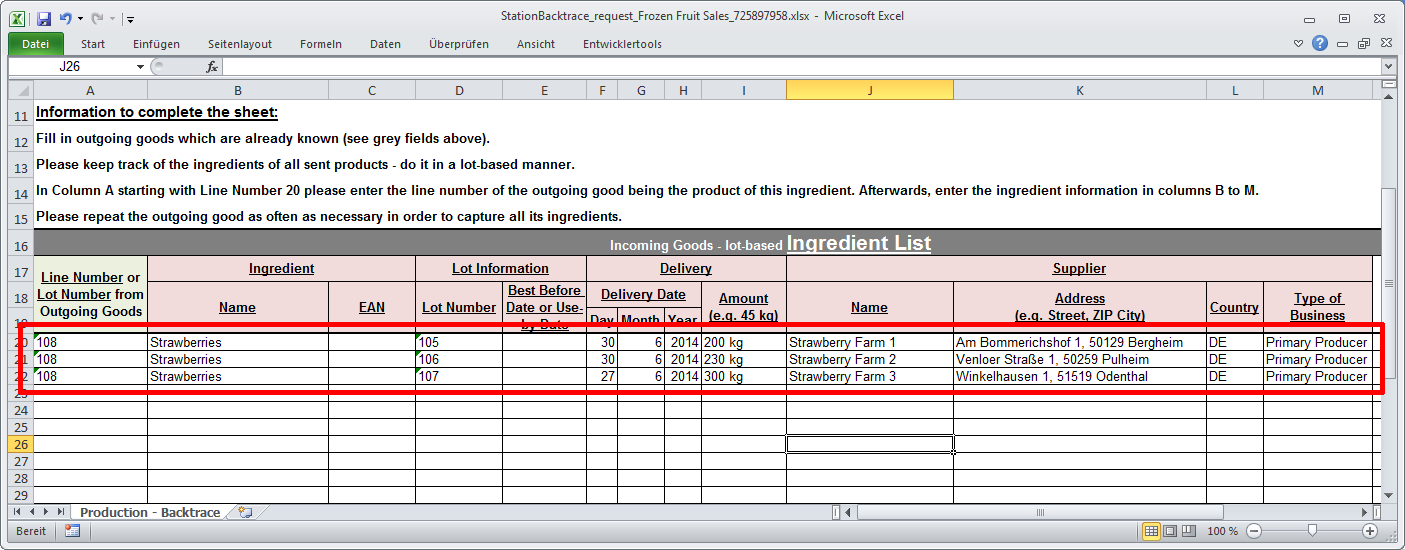
\includegraphics[width=0.95\textwidth]{7.png}
	\end{center}
	\begin{itemize}
		\item Now scroll down to the section where you can enter the ingredients.
		\item Enter the 3 deliveries, that were used as ingredients for lot "108" (marked by the red box).
		\item Save and close the document.
	\end{itemize}
\end{frame}

\subsection{8}
\begin{frame}
	\begin{center}
  		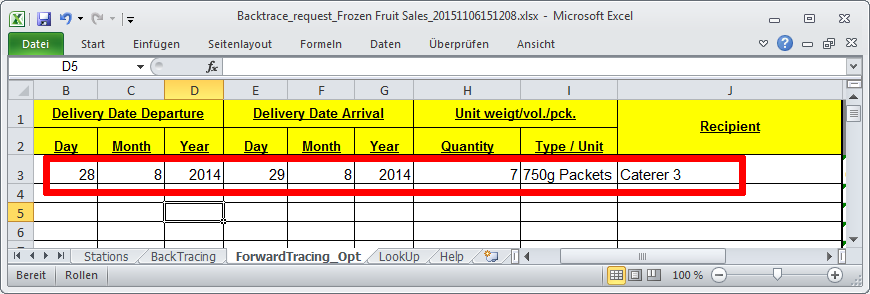
\includegraphics[width=0.95\textwidth]{8.png}
	\end{center}
	\begin{itemize}
		\item To import this file click on the \textbf{Table import} button in the upper left corner of the database interface.
	\end{itemize}
\end{frame}

\subsection{9}
\begin{frame}
	\begin{center}
  		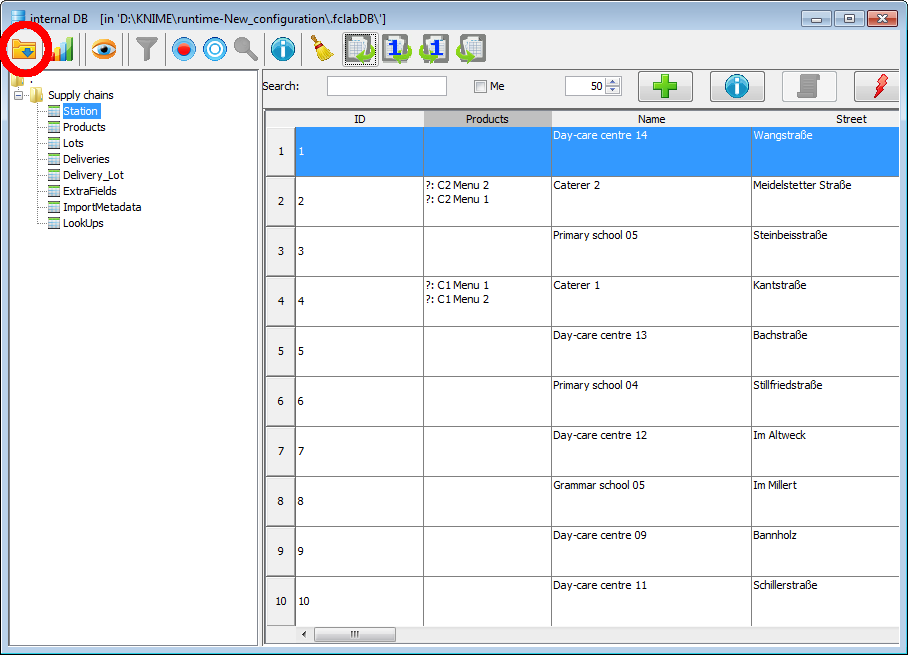
\includegraphics[height=0.6\textheight]{9.png}
	\end{center}
	\begin{itemize}
		\item In the file dialog that appears, select "StationBacktrace\_request\_Frozen Fruit Sales\_725897958..." and press \textbf{Open}.
	\end{itemize}
\end{frame}

\subsection{10}
\begin{frame}
	\begin{center}
  		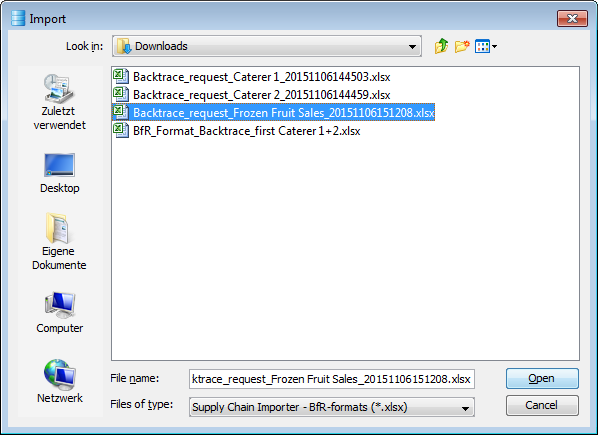
\includegraphics[height=0.2\textheight]{10.png}
	\end{center}
	\begin{itemize}
		\item You'll see a message that the import was successful.
		\item Press \textbf{OK}.
	\end{itemize}
\end{frame}

\subsection{11}
\begin{frame}
	\begin{center}
  		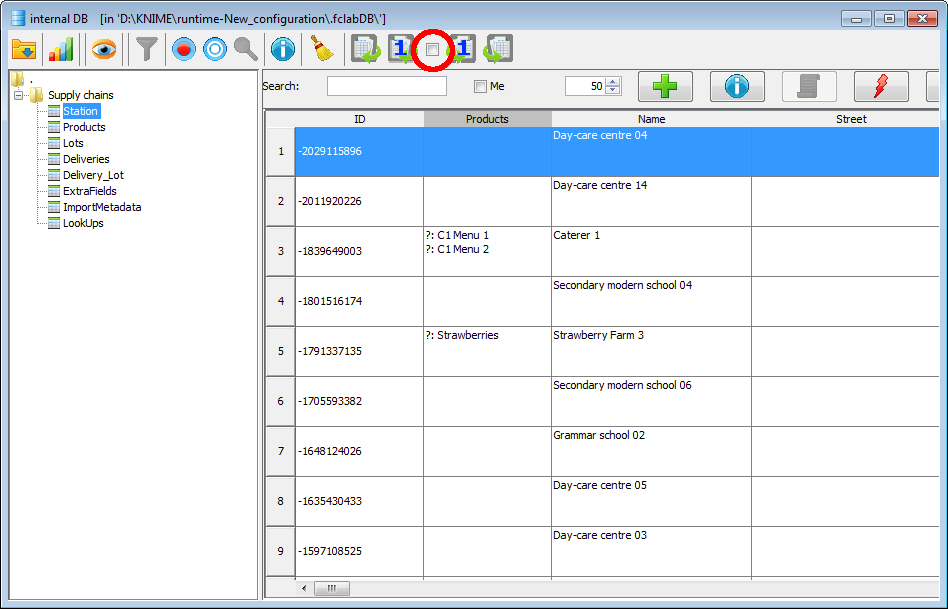
\includegraphics[height=0.4\textheight]{11.png}
	\end{center}
	\begin{itemize}
		\item The frozen strawberries from lot "108" were not only delivered to "Caterer 1" and "Caterer 2", but also to a third caterer.
		\item To get this information into the database we have to create a forward tracing template for "Frozen Fruit Sales".
		\item First we have to uncheck \textbf{Generate only the missing data}. Otherwise no template would be generated, since FoodChain-Lab assumes that no data is missing for lot "108" as its ingredients and the deliveries of the lot to "Caterer 1" and "Caterer 2" are already in the database.
	\end{itemize}
\end{frame}

\subsection{12}
\begin{frame}
	\begin{center}
  		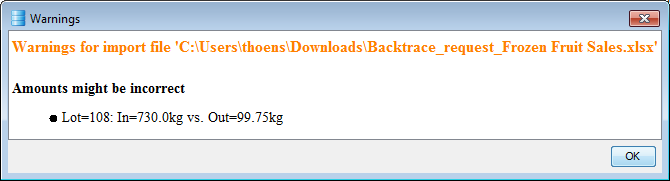
\includegraphics[width=0.95\textwidth]{12.png}
	\end{center}
	\begin{itemize}
		\item Press the button for generating a forward tracing template for one station, which is marked by the red circle.
	\end{itemize}
\end{frame}

\subsection{13}
\begin{frame}
	\begin{center}
  		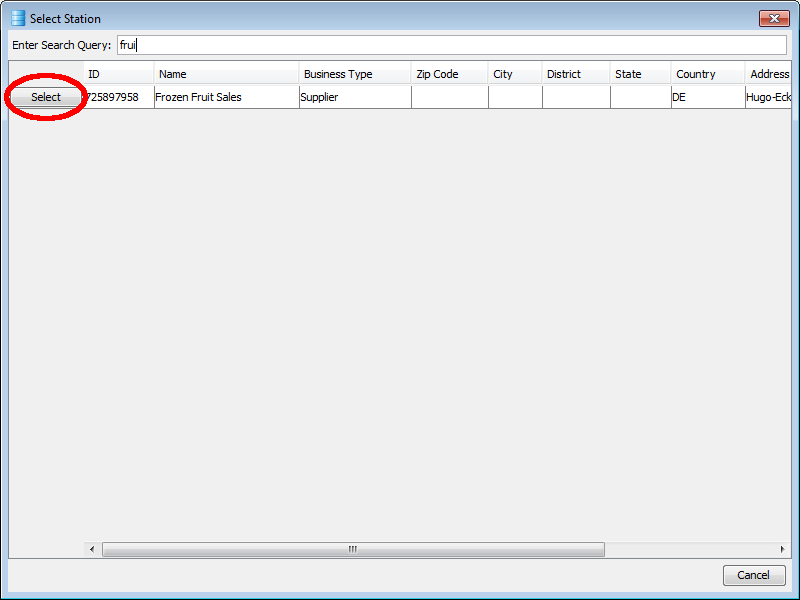
\includegraphics[height=0.6\textheight]{13.png}
	\end{center}
	\begin{itemize}
		\item In the dialog that appears search for "Frozen Fruit Sales" and click its \textbf{Select} button.
	\end{itemize}
\end{frame}

\subsection{14}
\begin{frame}
	\begin{center}
  		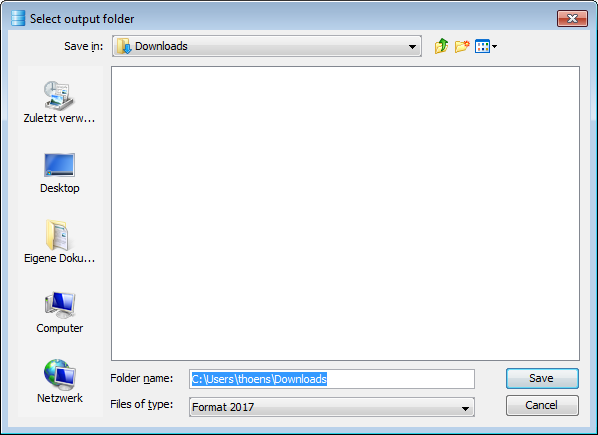
\includegraphics[height=0.6\textheight]{14.png}
	\end{center}
	\begin{itemize}
		\item In the file dialog that appears, you can specify the folder where the generated templates should be saved.
		\item Select the desired folder and press \textbf{Save}.
	\end{itemize}
\end{frame}

\subsection{15}
\begin{frame}
	\begin{center}
  		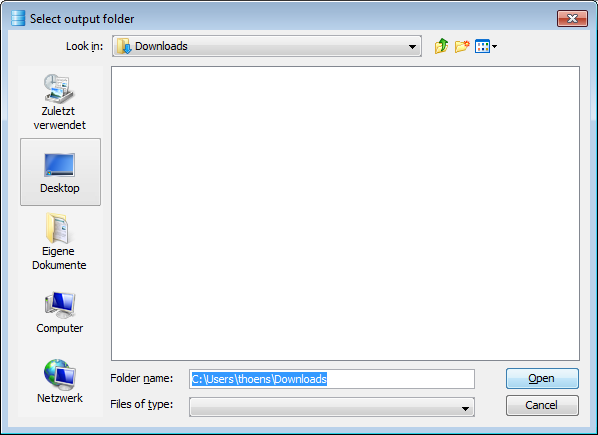
\includegraphics[height=0.2\textheight]{15.png}
	\end{center}
	\begin{itemize}
		\item You'll be noticed, that one template was generated in the folder you specified.
		\item Press \textbf{OK}.
	\end{itemize}
\end{frame}

\subsection{16}
\begin{frame}
	\begin{center}
  		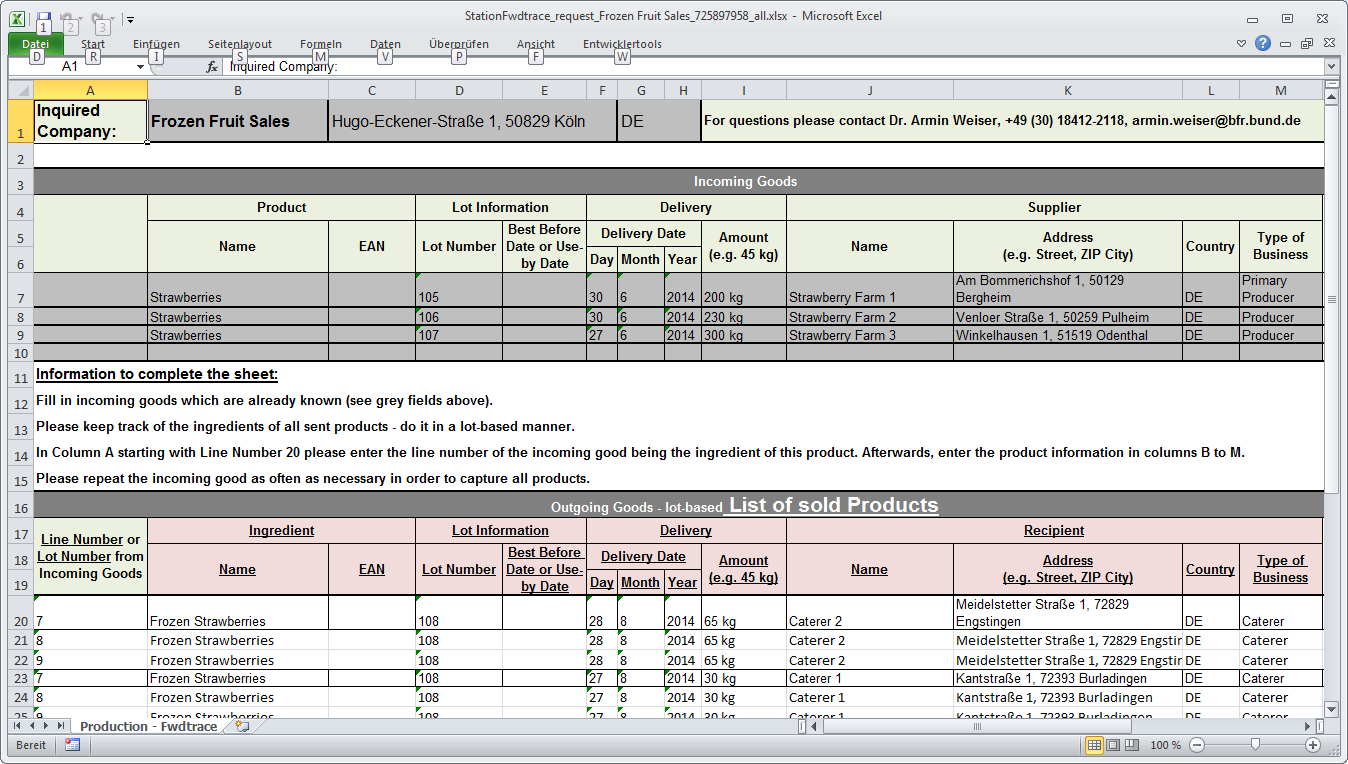
\includegraphics[width=0.8\textwidth]{16.png}
	\end{center}
	\begin{itemize}
		\item Open the generated template ("StationFwdtrace\_request\_Frozen Fruit Sales...").
		\item In the upper part you can see all incoming deliveries (ingredients) of "Frozen Fruit Sales".
	\end{itemize}
\end{frame}

\subsection{17}
\begin{frame}
	\begin{center}
  		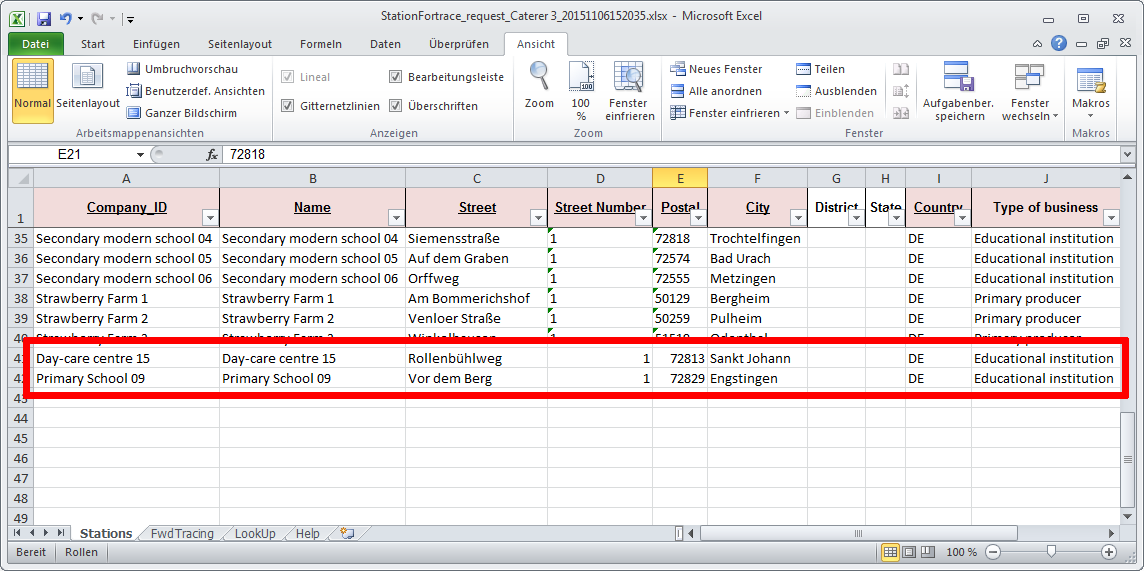
\includegraphics[height=0.5\textheight]{17.png}
	\end{center}
	\begin{itemize}
		\item Scroll down to the section where you can enter the outgoing deliveries.
		\item There was one delivery of "Frozen Strawberries" of lot "108" to "Caterer 3".
		\item Since lot "108" already exists, we do not have to define any ingredients and can leave the first cell empty.
		\item Enter the delivery as shown on the screenshot (red box).
		\item After entering the data save and close the document.
	\end{itemize}
\end{frame}

\subsection{18}
\begin{frame}
	\begin{center}
  		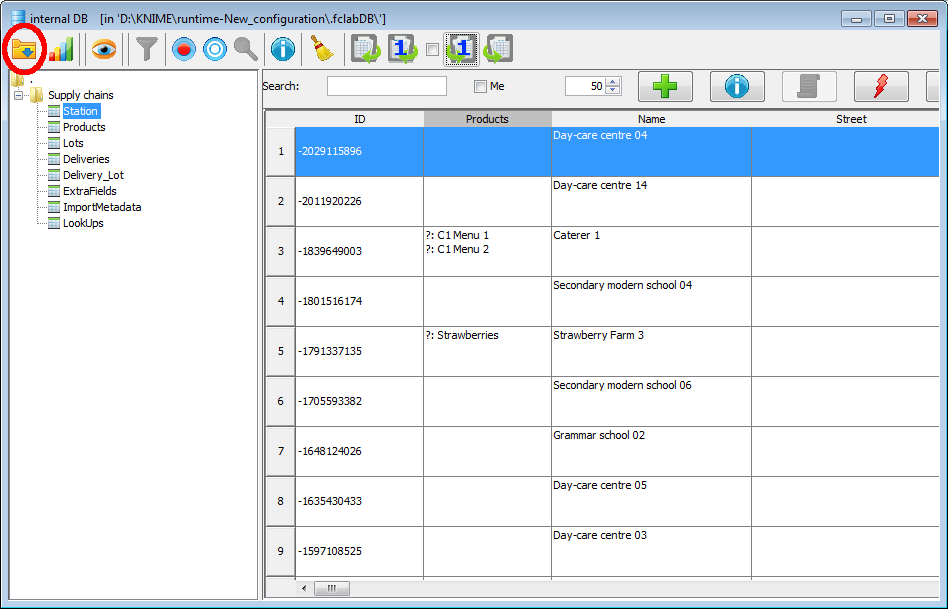
\includegraphics[width=0.9\textwidth]{18.png}
	\end{center}
	\begin{itemize}
		\item To import this file click on the \textbf{Table import} button in the upper left corner of the database interface.
	\end{itemize}
\end{frame}

\subsection{19}
\begin{frame}
	\begin{center}
  		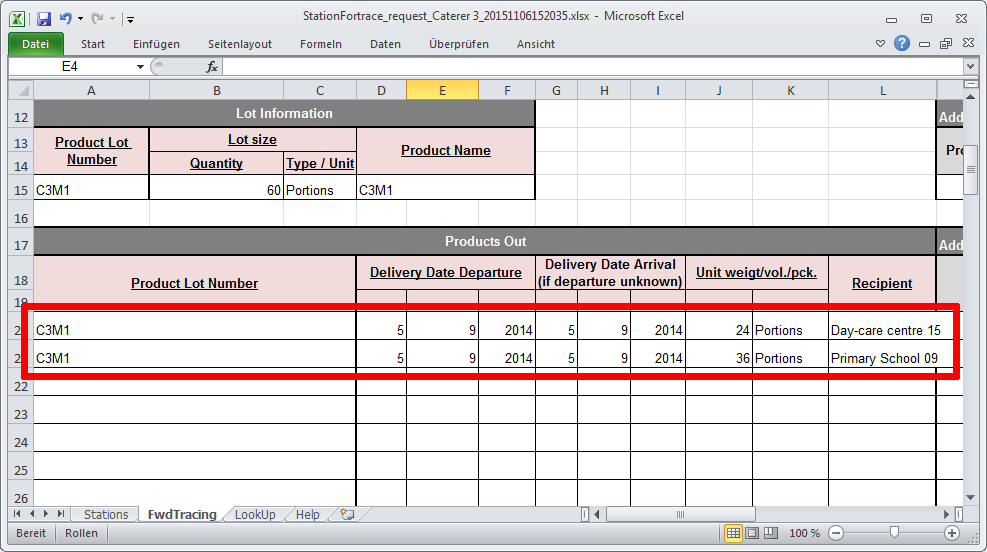
\includegraphics[height=0.5\textheight]{19.png}
	\end{center}
	\begin{itemize}
		\item In the file dialog that appears, select "StationFwdtrace\_request\_Frozen Fruit Sales..." and press \textbf{Open}.	
	\end{itemize}
\end{frame}

\subsection{20}
\begin{frame}
	\begin{center}
  		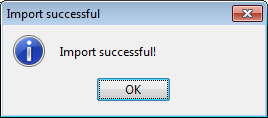
\includegraphics[height=0.2\textheight]{20.png}
	\end{center}
	\begin{itemize}
		\item You'll see a message that the import was successful.
		\item Press \textbf{OK}.
	\end{itemize}
\end{frame}

\end{document}